% VUT FIT MITAI
% MSZ 2021/2022
% Author: Vladimir Dusek
% Login: xdusek27

%%%%%%%%%%%%%%%%%%%%%%%%%%%%%%%%%%%%%%%%%%%%%%%%%%%%%%%%%%%%%%%%%%%%%%%%%%%%%%%%

% Path to figures
\graphicspath{{kry/symetricka_kryptografie/figures}}

%%%%%%%%%%%%%%%%%%%%%%%%%%%%%%%%%%%%%%%%%%%%%%%%%%%%%%%%%%%%%%%%%%%%%%%%%%%%%%%%

\chapter{KRY -- Symetrická kryptografie. Vlastnosti, vlastnosti bezpečného algoritmu, délka klíče, útok silou, příklady symetrických algoritmů, Feistelovy šifry, DES, režimy činnosti, proudové šifry.}

%%%%%%%%%%%%%%%%%%%%%%%%%%%%%%%%%%%%%%%%%%%%%%%%%%%%%%%%%%%%%%%%%%%%%%%%%%%%%%%%

\section{Metadata}

\begin{compactitem}
    \item Předmět: Kryptografie (KRY)
    \item Přednáška:
    \begin{compactitem}
        \item 3) Symetrická kryptografie. Vlastnosti, vlastnosti bezpečného algoritmu, délka klíče, útok silou.
        \item 4) Příklady symetrických algoritmů, Feistelovy šifry, DES, struktura, činnost, slabiny, režimy činnosti.
        \item 5) Typické aplikace symetrické kryptografie.
    \end{compactitem}
    \item Záznam:
    \begin{compactitem}
        \item 2021-02-22
        \item 2021-03-01
        \item 2021-03-08
    \end{compactitem}
\end{compactitem}

%%%%%%%%%%%%%%%%%%%%%%%%%%%%%%%%%%%%%%%%%%%%%%%%%%%%%%%%%%%%%%%%%%%%%%%%%%%%%%%%

\section{Úvod a kontext}

\paragraph*{Kryptografie} Kryptografie (šifrování) je věda o~metodách utajování smyslu zpráv převodem do podoby, která je čitelná jen se speciální znalostí.

\paragraph*{Kryptoanalýza} Kryptoanalýza je věda zabývající se metodami získávání obsahu šifrovaných informací bez přístupu k~tajným informacím, které jsou za normálních okolností potřeba, tzn. především k~tajnému klíči.

\paragraph*{Kryptologie} Jeden výraz pro kryptografii a kryptoanalýzu.

\paragraph*{Caesarova šifra} Princip Caesarovy šifry je založen na tom, že všechna písmena zprávy jsou během šifrování zaměněna za písmeno, které se abecedně nachází o~pevně určený počet míst dále (tj. posun je pevně zvolen). Caesarova šifra spadá do kategorie substitučních šifer (stejný znak je při více vyskytech vždy zašifrován na stejný znak).

\paragraph*{Vigenerova šifra} Rozšíření Caesarovy šifry, klíč je delší než 1 znak. Klíč je řetězec, který reprezentuje posuny. V~případě že vstup je delší než klíč, je klíč perioricky opakován. Vigenerova šifra spadá do kategorie polyalfabetických substitučních šifer (stejný znak může být při více výskytech zašifrován na jiný znak).

\paragraph*{Vernamova šifra (\textit{One Time Pad})} Vernamova šifra spadá do kategorie polyalfabetických substitučních šifer a je i dnes nerozluštitelná pokud: \begin{compactitem}
    \item klíč je delší než vstupní text,
    \item klíč se nepoužije opakovaně,
    \item klíč je náhodný.
\end{compactitem}

\begin{figure}[H]
    \centering
    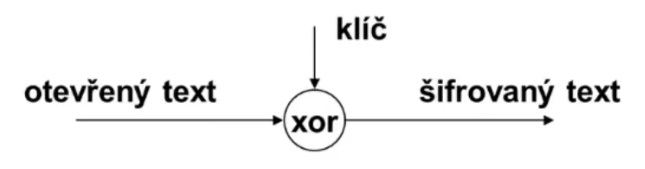
\includegraphics[width=0.5\linewidth]{vernam.png}
    \caption{Vernamova šifra.}
\end{figure}

\paragraph*{Autoklíč (\textit{autokey})} Šifrování klíčem a když vstupní text je delší než klíč, tak se pokračuje šifrováním otevřeným nebo šifrovaným textem. Lze použít u~Vigenerovy nebo Vernamovy šifry.

\paragraph*{Symetrická kryptografie} Algoritmy používají k~šifrování i dešifrování stejný klíč. Výhodou symetrických šifer je jejich nízká výpočetní náročnost. Asymetrické šifry mohou být i stotisíckrát pomalejší. Nevýhodou je nutnost sdílení tajného klíče, takže jedna strana musí klíč vygenerovat a potom ho bezpečným způsobem předat druhé straně.

\paragraph*{Typy útoků} \begin{compactitem}
    \item Ciphertext Only Attack (COA) -- Útočník zná pouze zašifrovaný text a snaží se zjistit klíč nebo otevřený text. Nejčastěší případ.
    \item Known Plaintext Attack (KPA) -- Útočník zná zašifrovaný text a otevřený text a snaží se zjistit klíč.
    \item Chosen Plaintext Attack (CPA) -- Útočník zná to co v~KPA a navíc si text může zvolit.
\end{compactitem}

\paragraph*{Útok silou} Pří útoku silou (\textit{brute force}) zkouší útočník všechny teoreticky možné klíče, dokud nenajde ten správný.

\begin{figure}[H]
    \centering
    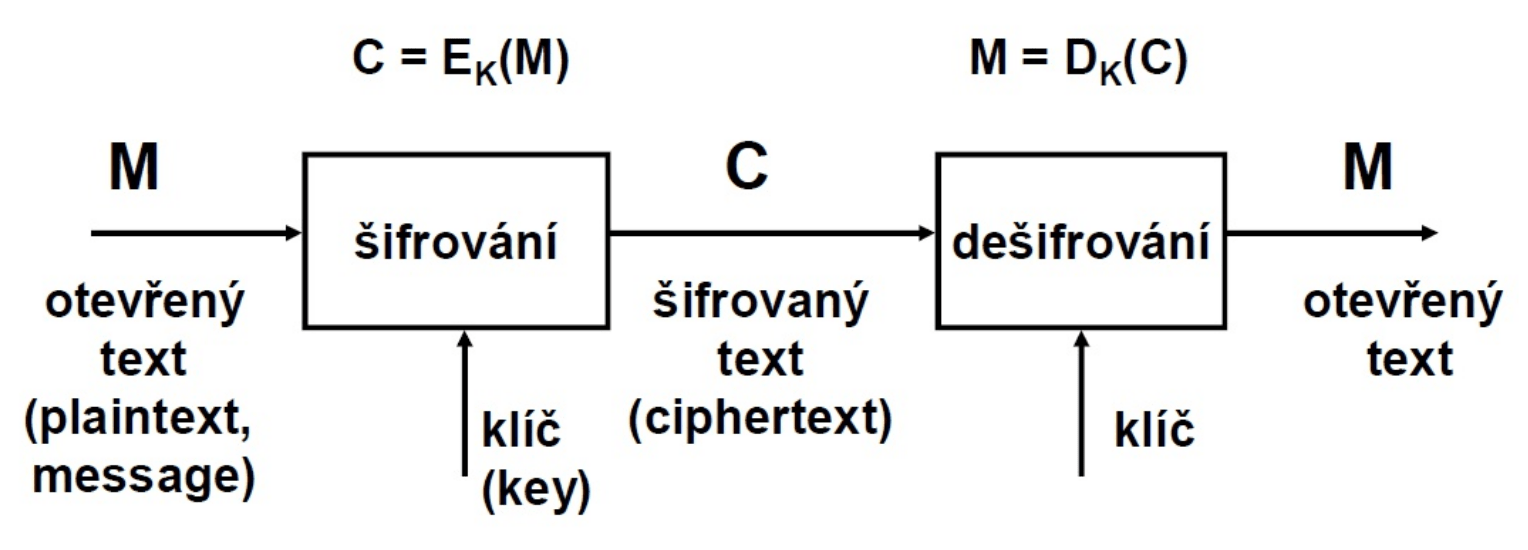
\includegraphics[width=0.75\linewidth]{kryptografie.png}
    \caption{Princip kryptografie, podle typu klíčů dělíme na symetrickou (tajný klíč) a asymetrickou (veřejný klíč, soukromý klíč).}
\end{figure}

\paragraph*{Bezpečný algoritmus} V~moderní kryptografii je nepřijatelné utajování algoritmů (\textit{security by obscurity})~--~předpokládáme, že útočník zná šifrovací algoritmus. Bezpečnost musí záviset pouze na utajení klíče (Kerckhoffuv princip, \textit{security by design}). Symetrický algoritmus je považován za bezpečný, pokud neexistuje rychlejší útok než útok silou.

\paragraph*{Délka klíče} Dnes je považováno 80 bitů a více za dostatečné. Typicky se délka zaokrouhluje na mocninu 2 (typicky 128b). Klíče symetrických algoritmů jsou kratší než asymetrických. Konkrétně: DES -- 56b, 3DES -- 112, AES -- variabilní.

\paragraph*{Využití} Symetrická kryptografie je vhodná pro šifrování většího objemu dat. Narozdíl od asymetrické, která je pro tento účel příliš pomalá. Proto např. HTTPS využívá asymetrickou kryptografii pro výměnu symetrických klíčů a poté symetrickou kryptografii pro šifrování provozu.

\paragraph*{Vlastnosti moderní kryptografie} Symetrická kryptografie zaručuje všechny následující, kromě nepopiratelnosti~--~více entit má k~dispozici klíč. \begin{compactitem}
    \item Důvernost -- Utajení informace. Bez znalosti klíče, není možné data číst.

    \item Autentizace -- Prokázání, že zprávu skutečně poslal odesílatel a nikoliv útočník, který se za odesílatele vydává.

    \item Integrita -- Prokázání, že nikdo nemohl data po cestě od odesílatele k~příjemci změnit. Ochrana proti neoprávněné, neodhalené modifikaci zprávy.

    \item Nepopiratelnost -- Pokud odesílatel data poslal, nemůže tuto skutečnost popřít.
\end{compactitem}

%%%%%%%%%%%%%%%%%%%%%%%%%%%%%%%%%%%%%%%%%%%%%%%%%%%%%%%%%%%%%%%%%%%%%%%%%%%%%%%%

\section{Blokové šifry}

Blokové šifry šifrují data po blocích pevně stanovené délky (64b, 128b, 256b, \dots). Pokud je dat více, rozdělí se na více bloků, přičemž do zbylého místa v~posledním je umístěno zarovnání \textit{padding} (informace o~délce zarovnání může být obsažena v~posledním bytu). Příklady blokových šifer: \begin{compactitem}
    \item Feistelova šifra (spíše princip)
    \item Data Encryption Standard (DES)
    \item Triple Data Encryption Algorithm (3DES)
    \item International Data Encryption Algorithm (IDEA)
    \item Blowfish
    \item Tiny Encryption Algorithm (TEA)
    \item Advanced Encryption Standard (AES)
\end{compactitem}

\begin{figure}[H]
    \centering
    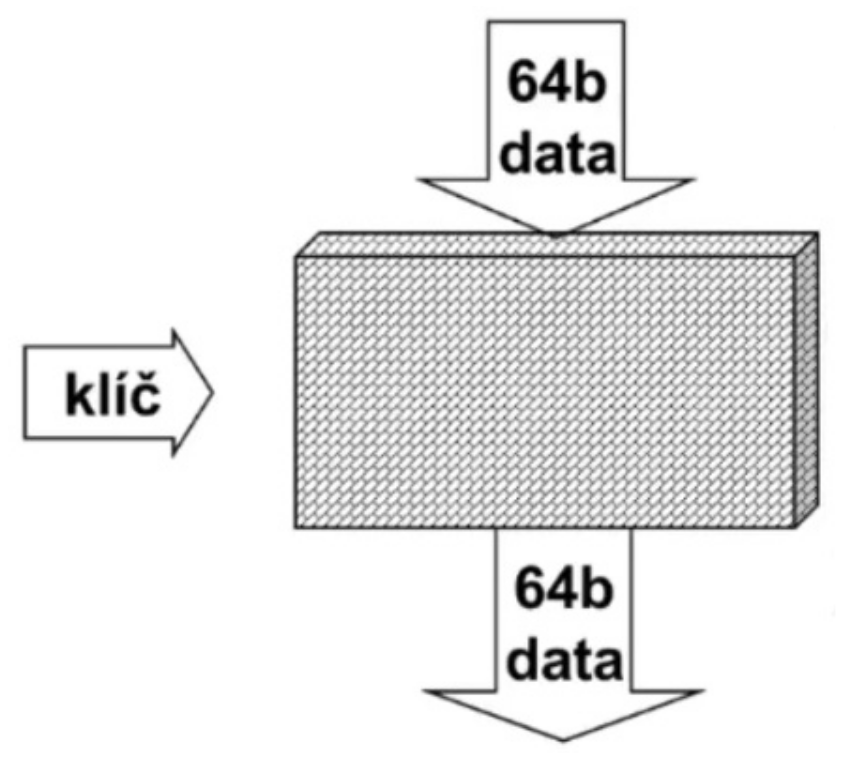
\includegraphics[width=0.35\linewidth]{symmetric_cryptography_blocks.png}
    \caption{Princip blokových šifer.}
\end{figure}

\subsection{Feistelova šifra}

Feistelova šifra (Feistelův princip) je koncept šifrování, který konkrétní algoritmy využívají. Jedná se o~substituční-permutační síť. Vstupní blok je rozdělen na dvě poloviny $L$ a $R$, výpočet výstupu pak vypadá následovně.

\begin{equation}
    L_i = R_{i-1}
\end{equation}

\begin{equation}
    R_i = L_{i-1} \oplus F(R_{i-1}, K_i)
\end{equation}

\paragraph*{Funkce F} $F$ je funkce, na kterou Feistelova šifra neklade žádné požadavky. Jednotlivé algoritmy, využívající Festelovu šifru, funkci samy definují. Požadavky na funkci $F$, aby algoritmus byl bezpečný: \begin{compactitem}
    \item skrytí vlastností zprávy;
    \item skrytí vlastností zprávy.
\end{compactitem}

\paragraph*{Subklíč} K~je tzv. subklíč, který je generován typicky nějakým pseudonáhodným generátorem na základě inicializačního klíče (hlavní).

\paragraph*{Dešifrování} Dešifrování se provádí stejným způsobem, pouze pořadí subklíčů je opačné.

\begin{figure}[H]
    \centering
    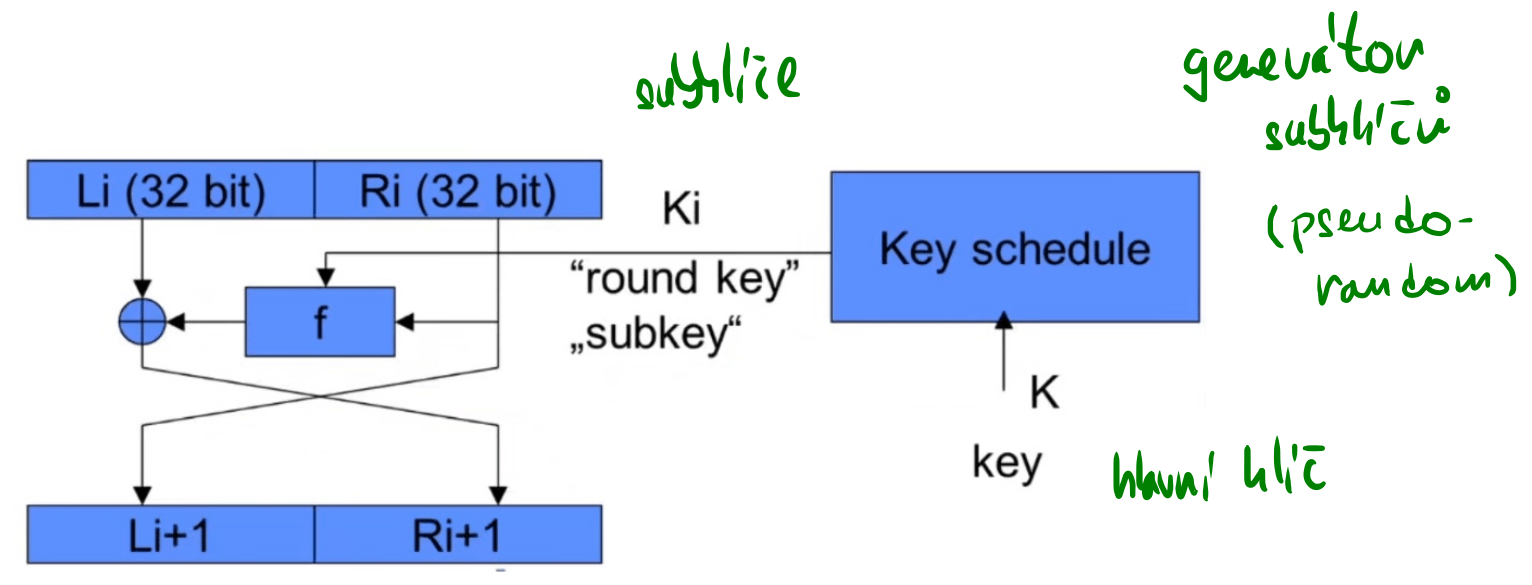
\includegraphics[width=1\linewidth]{feistel.png}
    \caption{Jeden krok opakování (Feistelův krok) vizuálně.}
\end{figure}

\begin{figure}[H]
    \centering
    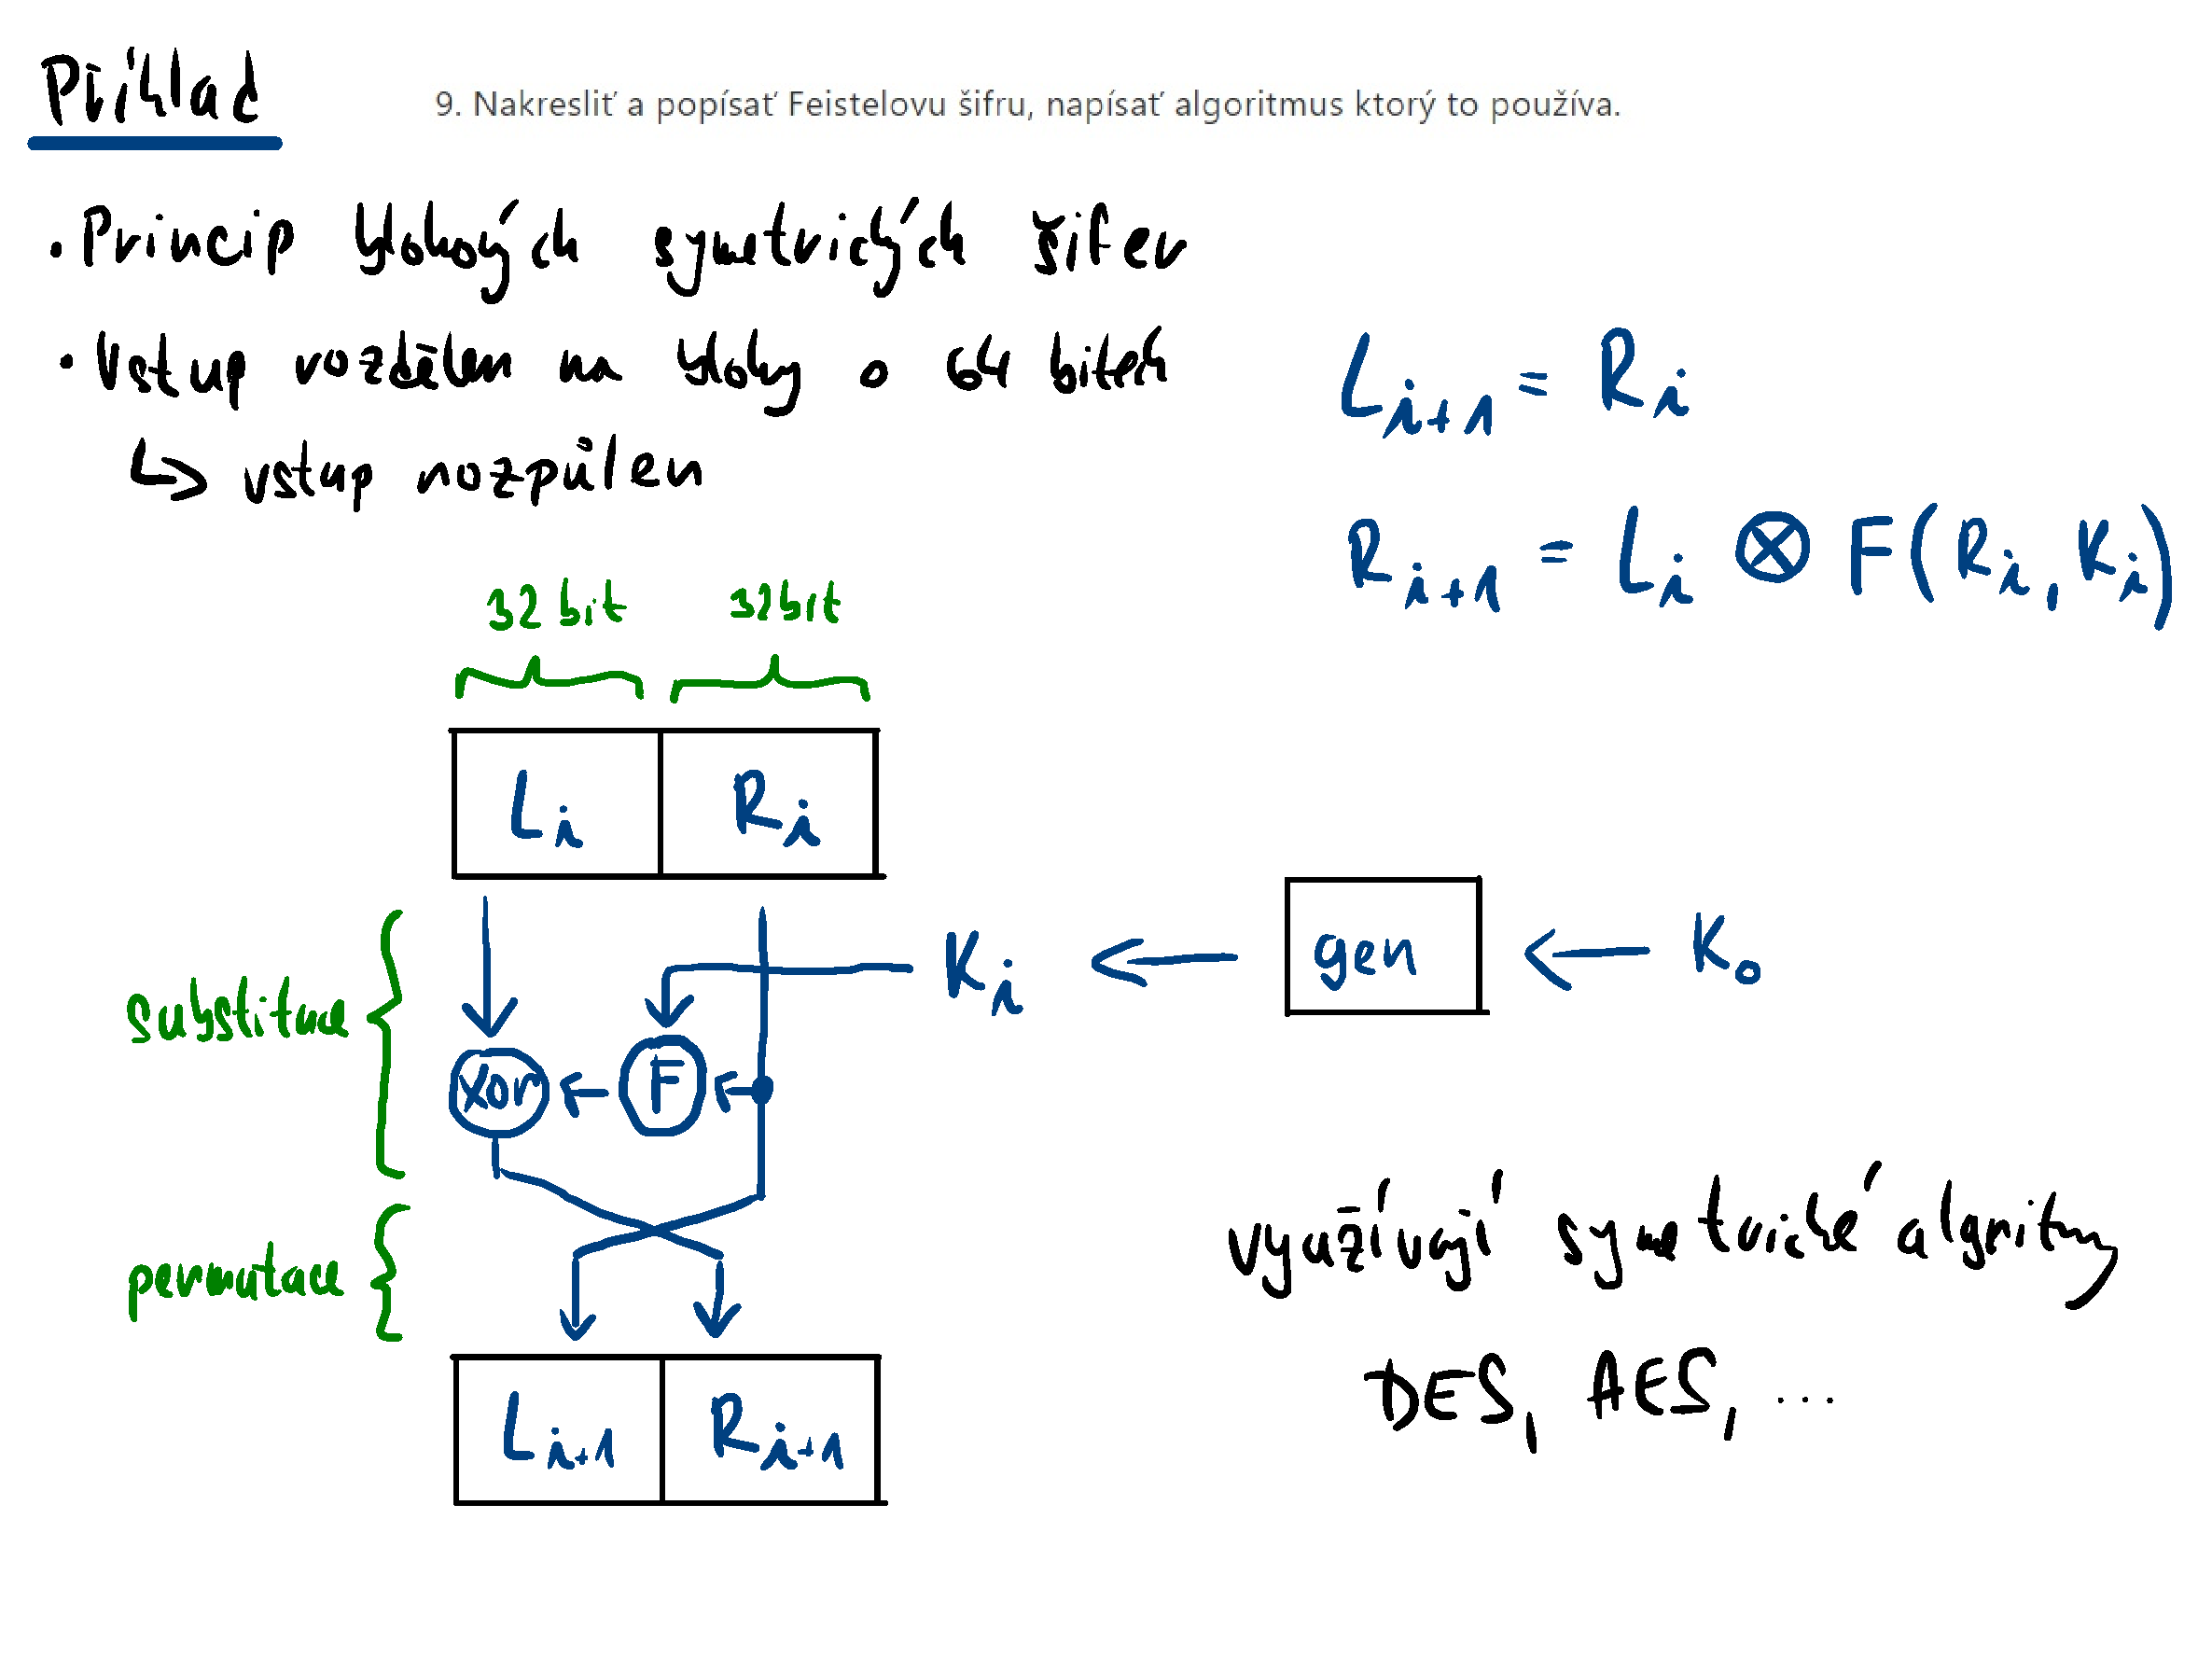
\includegraphics[width=1\linewidth]{feistel_example.pdf}
    \caption{Feistelova šifra -- příklad a rekapitulace.}
\end{figure}

\subsection{Data Encryption Standard (DES)}

DES byl první algoritmus s~veřejnou specifikací (\textit{security by design}). Využívá princip Feistelovy šifry -- 16 kol. Dodatečně přidává na začátek a konec permutaci navíc. Klíč je dlouhý 64b (resp. 56 významových bitů a 8 paritních).

\paragraph*{Slabiny} \begin{compactitem}
    \item 56 bitový klíč je příliš krátky a je možný útok silou.
    \item Rozdílná velikost bloku a klíče (zvláštnost).
    \item Existence slabých a poloslabých klíčů.
    \item Není jasné proč zrovna 16 iterací a zda je to dostatečné.
\end{compactitem}

\begin{figure}[H]
    \centering
    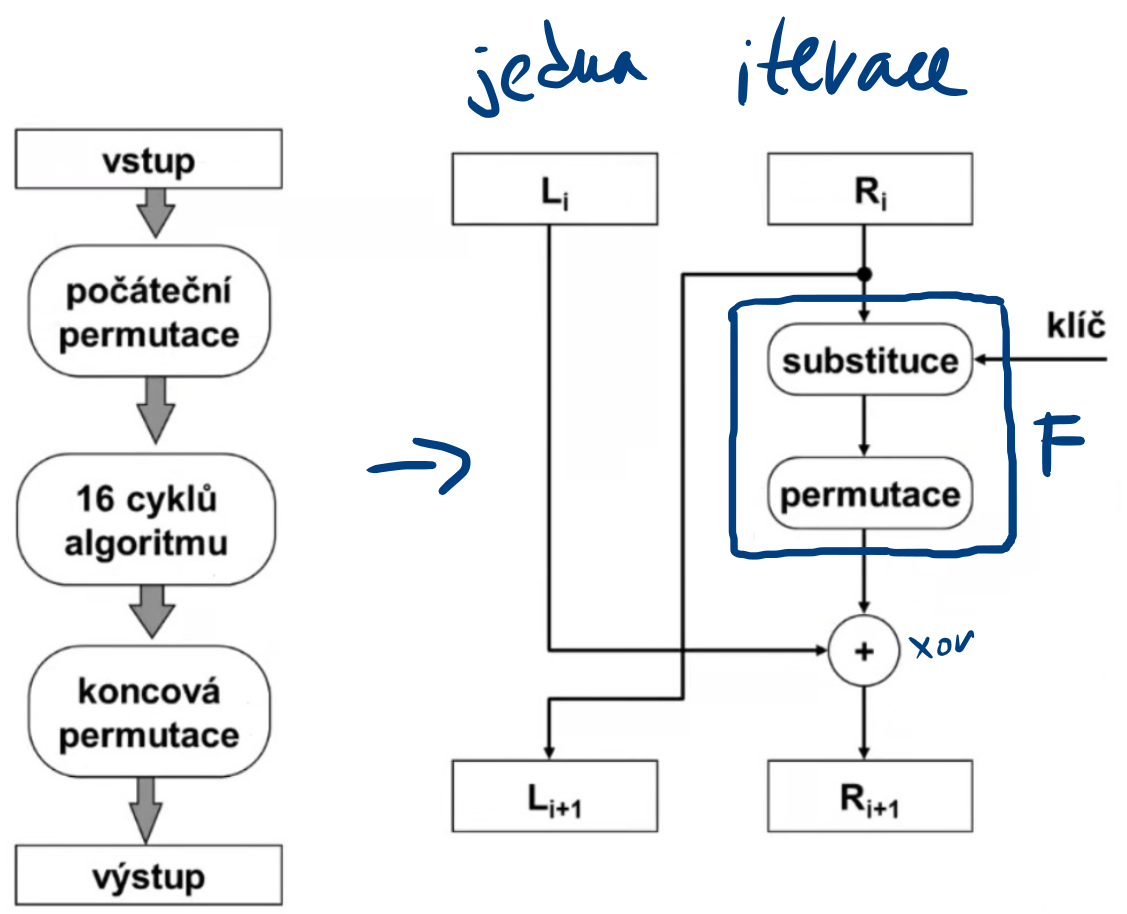
\includegraphics[width=0.75\linewidth]{des_schema.png}
    \caption{DES -- Schéma fungování algoritmu.}
\end{figure}

\begin{figure}[H]
    \centering
    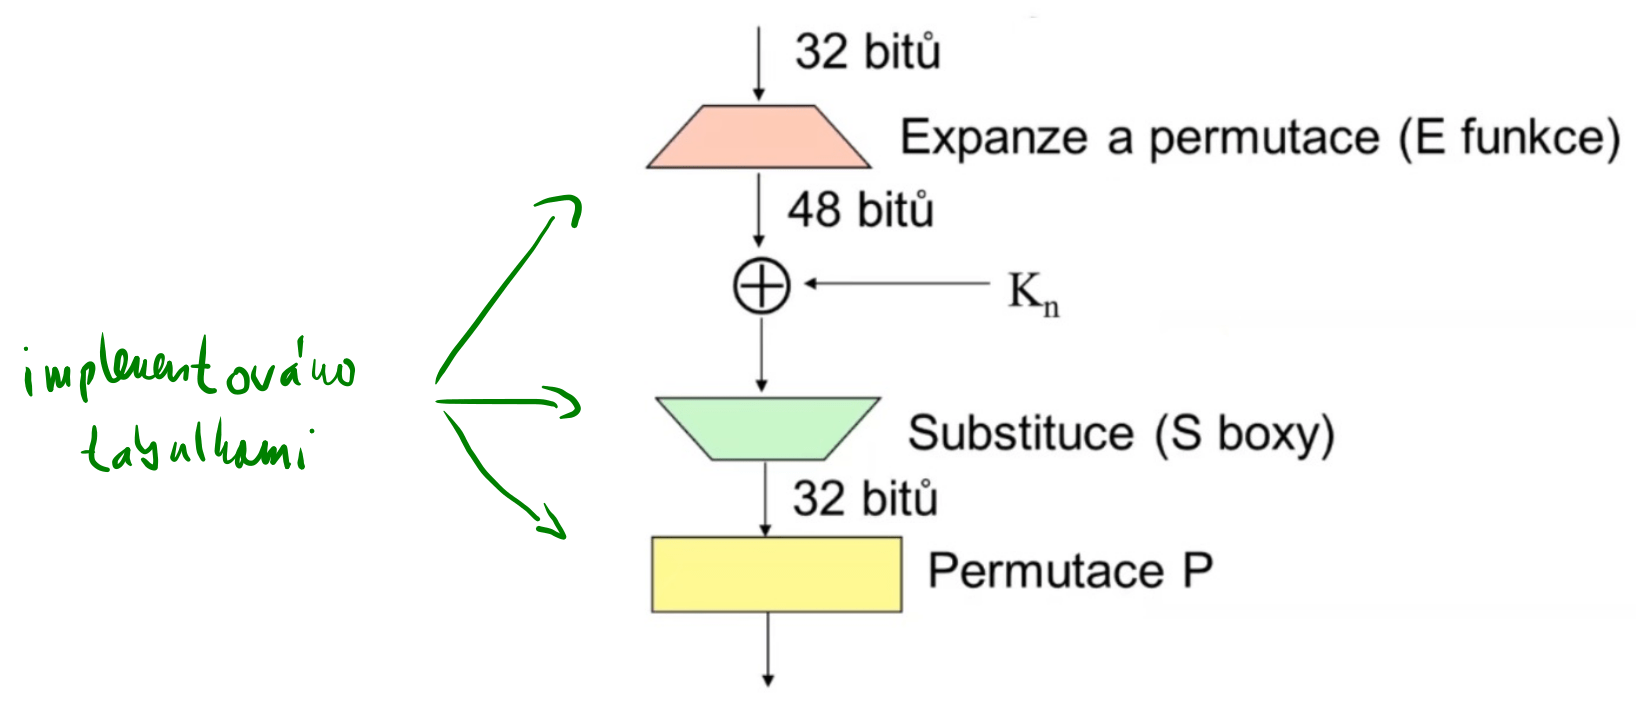
\includegraphics[width=1\linewidth]{des_f.png}
    \caption{DES -- funkce F.}
\end{figure}

\begin{figure}[H]
    \centering
    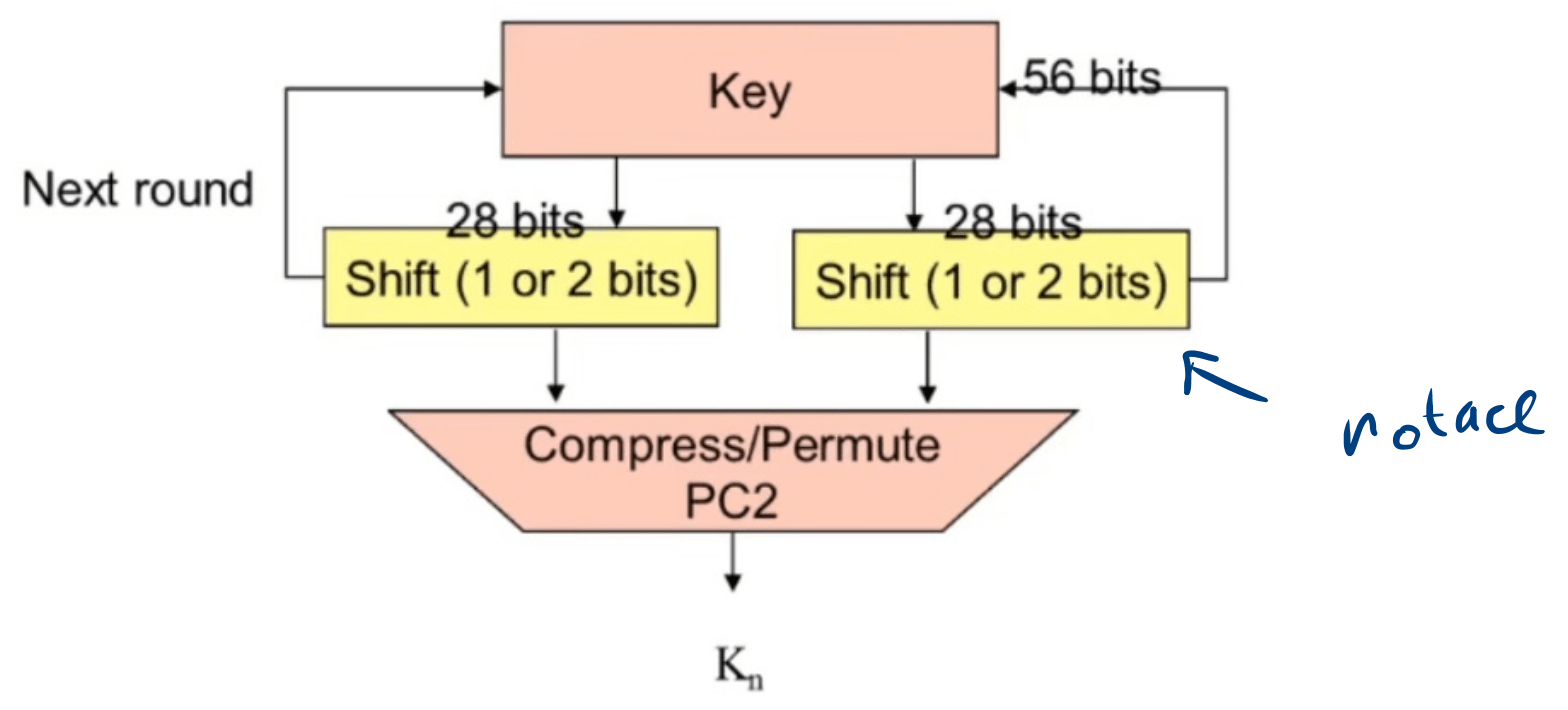
\includegraphics[width=1\linewidth]{des_keys.png}
    \caption{DES -- generování subklíčů.}
\end{figure}

\begin{figure}[H]
    \centering
    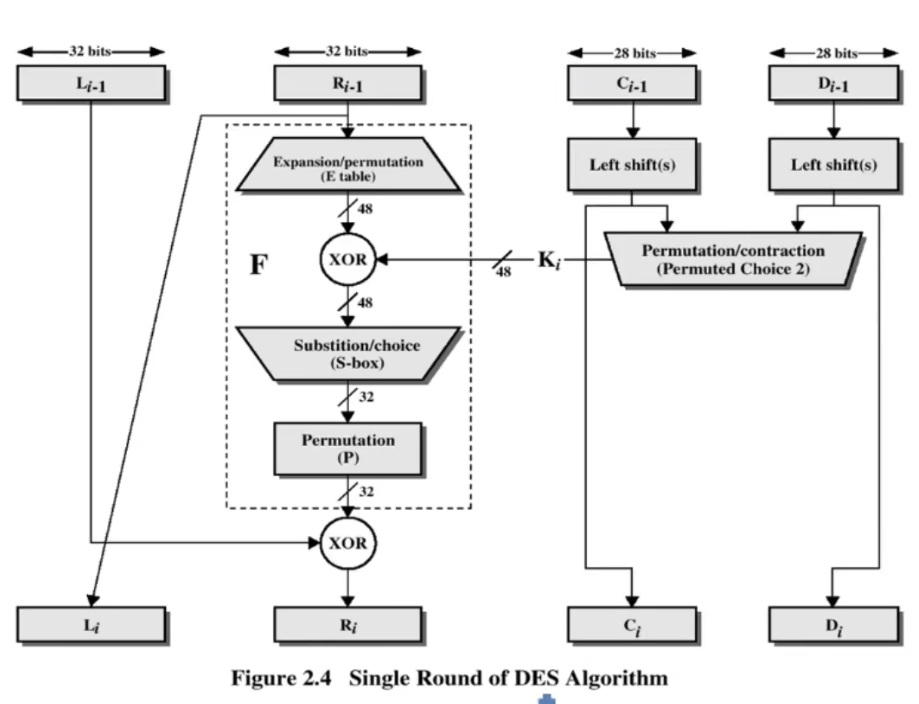
\includegraphics[width=1\linewidth]{des_single_round.png}
    \caption{DES -- jedno kolo algoritmu. \textit{Left shift} je ve skutečnosti bitová rotace.}
\end{figure}

\begin{figure}[H]
    \centering
    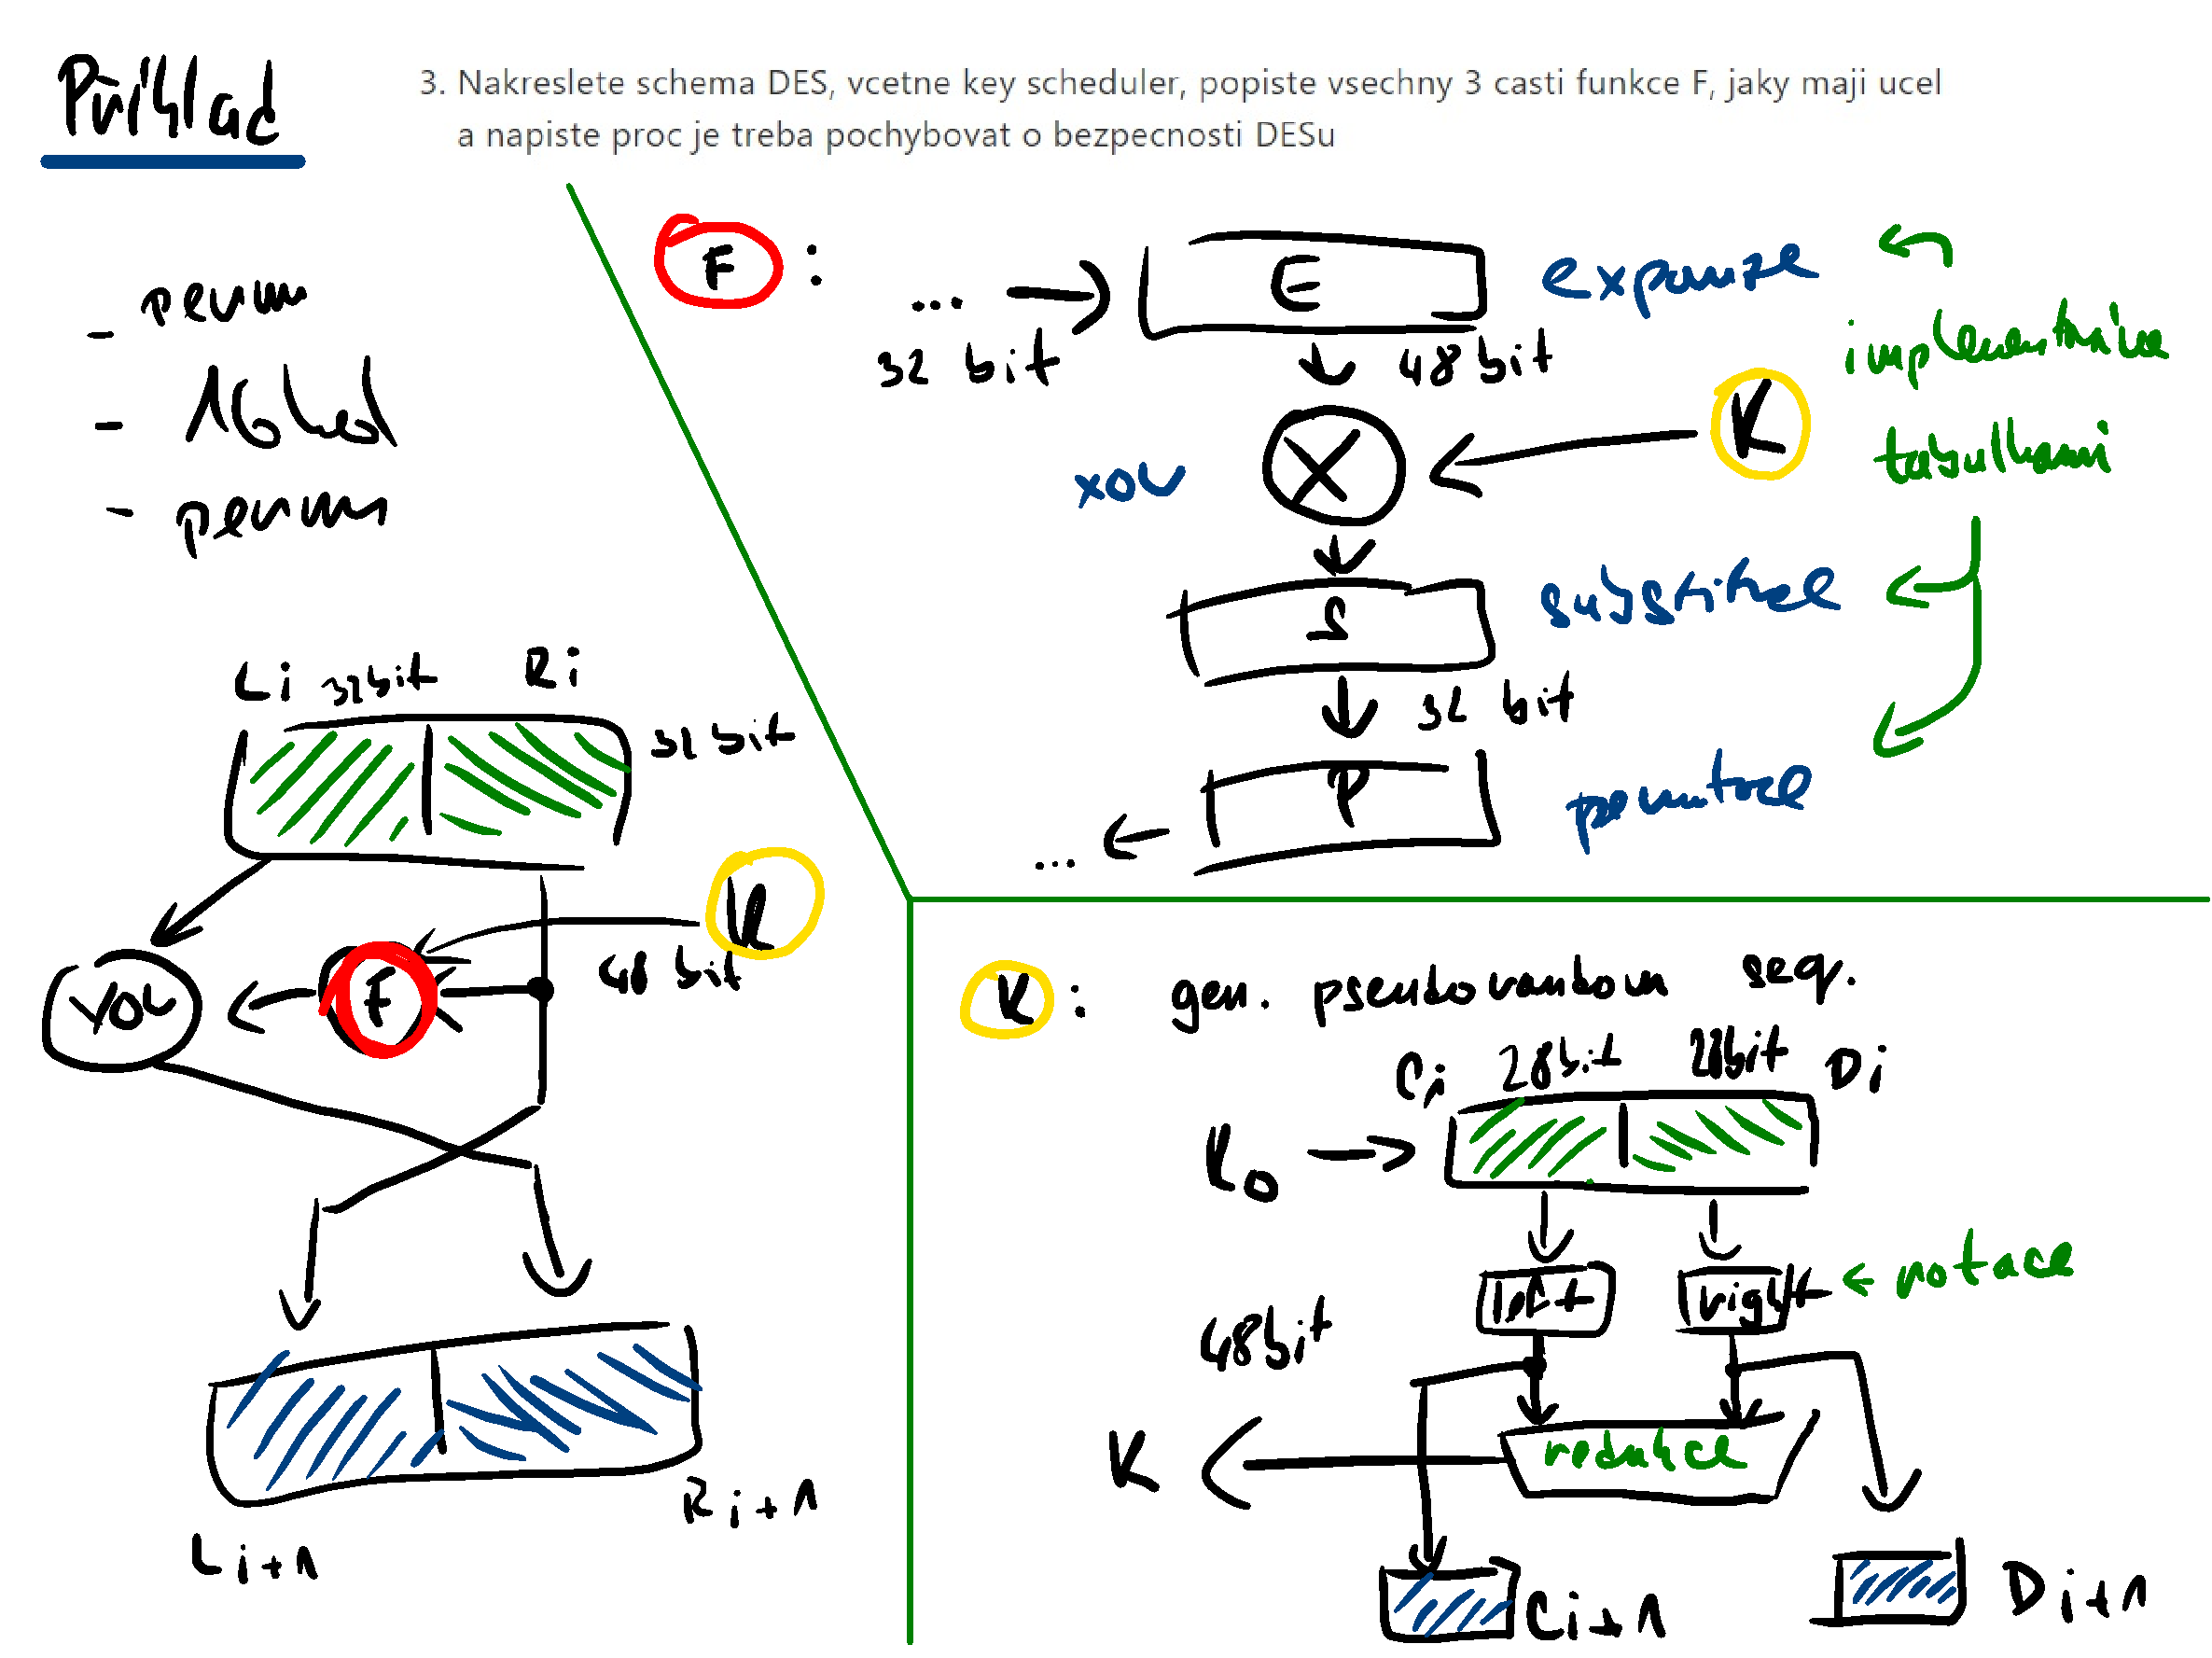
\includegraphics[width=1\linewidth]{des_example.pdf}
    \caption{DES -- příklad a rekapitulace.}
\end{figure}

%%%%%%%%%%%%%%%%%%%%%%%%%%%%%%%%%%%%%%%%%%%%%%%%%%%%%%%%%%%%%%%%%%%%%%%%%%%%%%%%

\section{Provozní režimy činnosti blokových šifer}

Jak použít blokové šifry abychom byli schopni šifrovat data delší než jeden blok?

\subsection{Electronic Code Book (ECB)}

ECB (\uv{kódová kniha}) je výchozí \textit{naivní} režim. Bloková šifra se při něm přímo aplikuje nezávisle na jednotlivé bloky, tedy při daném klíči odpovídá stejnému bloku otevřeného textu stejný blok šifrového textu. To má nežádoucí důsledky z~hlediska bezpečnosti, v~datech zůstane původní struktura, např. šifrovaný obrázek je rozpoznatelný.

\begin{figure}[H]
    \centering
    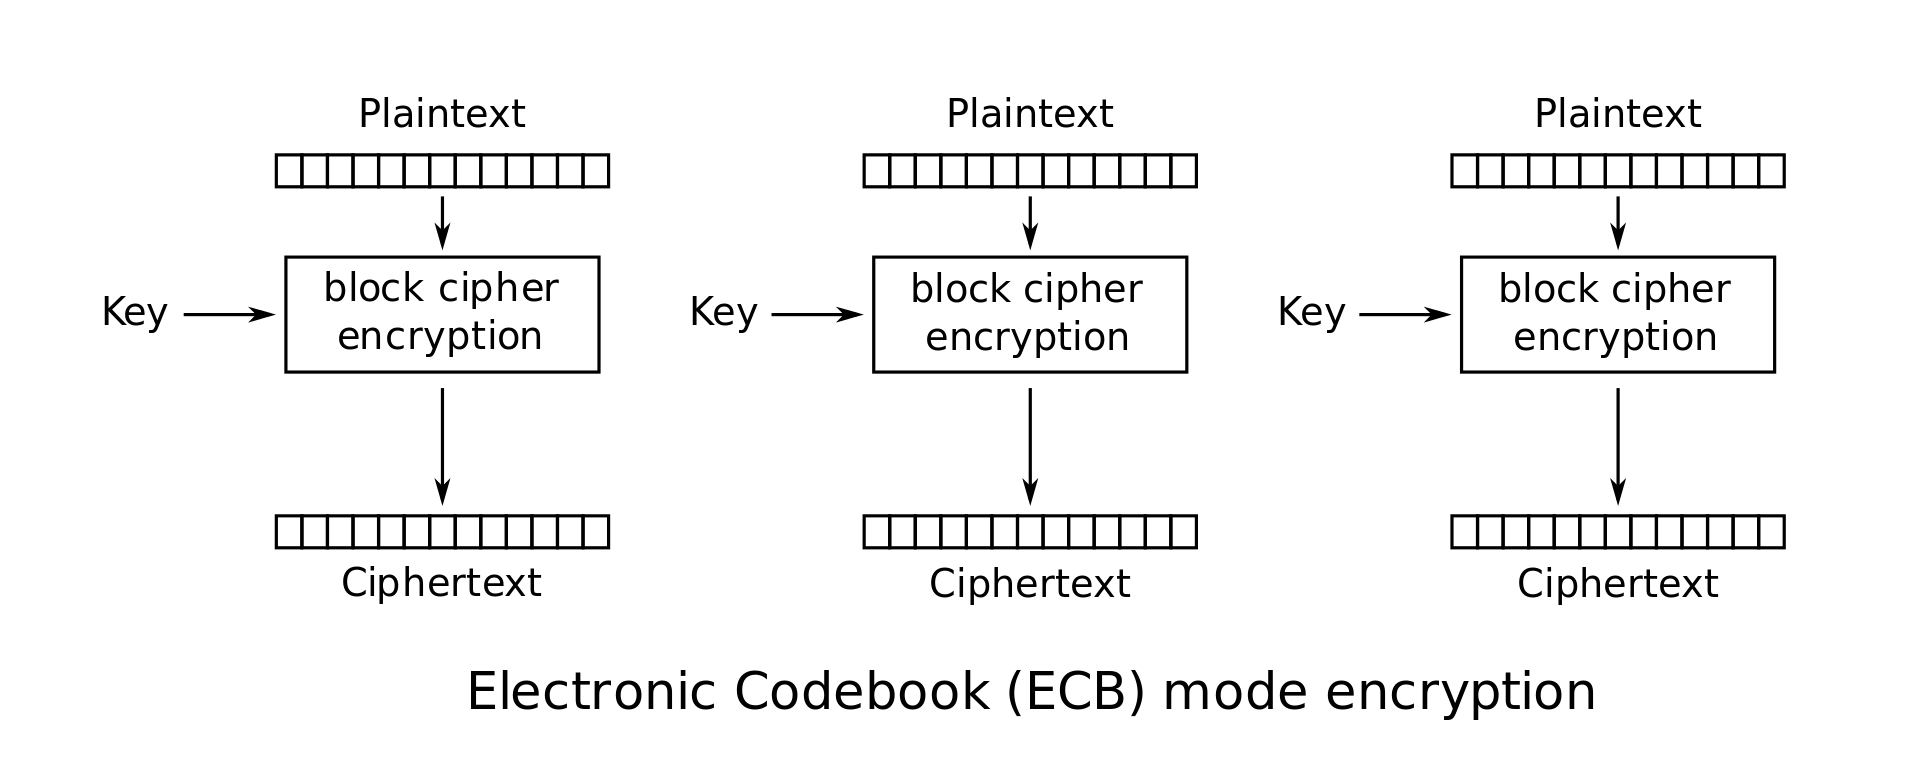
\includegraphics[width=1\linewidth]{rezim_ecb.png}
    \caption{Ukázka režimu ECB.}
\end{figure}

\subsection{Cipher Block Chaining (CBC)}

V~režimu CBC (\uv{řetězení šifrových bloků}) je každý blok před šifrováním xorován zašifrovaným předchozím blokem a první blok je xorován inicializačním vektorem. Tento režim je široce používán. Nevýhody plynou ze zřetězené závislosti (šifrovaný blok závisí na všech předcházejících): Šifrování nelze paralelizovat a při poškození šifrového bloku nelze dešifrovat ani blok přímo následující. Dešifrování paralelizovat lze.

\begin{equation}
\begin{aligned}
C_i &= E_K (P_i \oplus C_{i-1}) \\
P_i &= D_K(C_i) \oplus C_{i-1} \\
C_0 &= IV
\end{aligned}
\end{equation}

\begin{figure}[H]
    \centering
    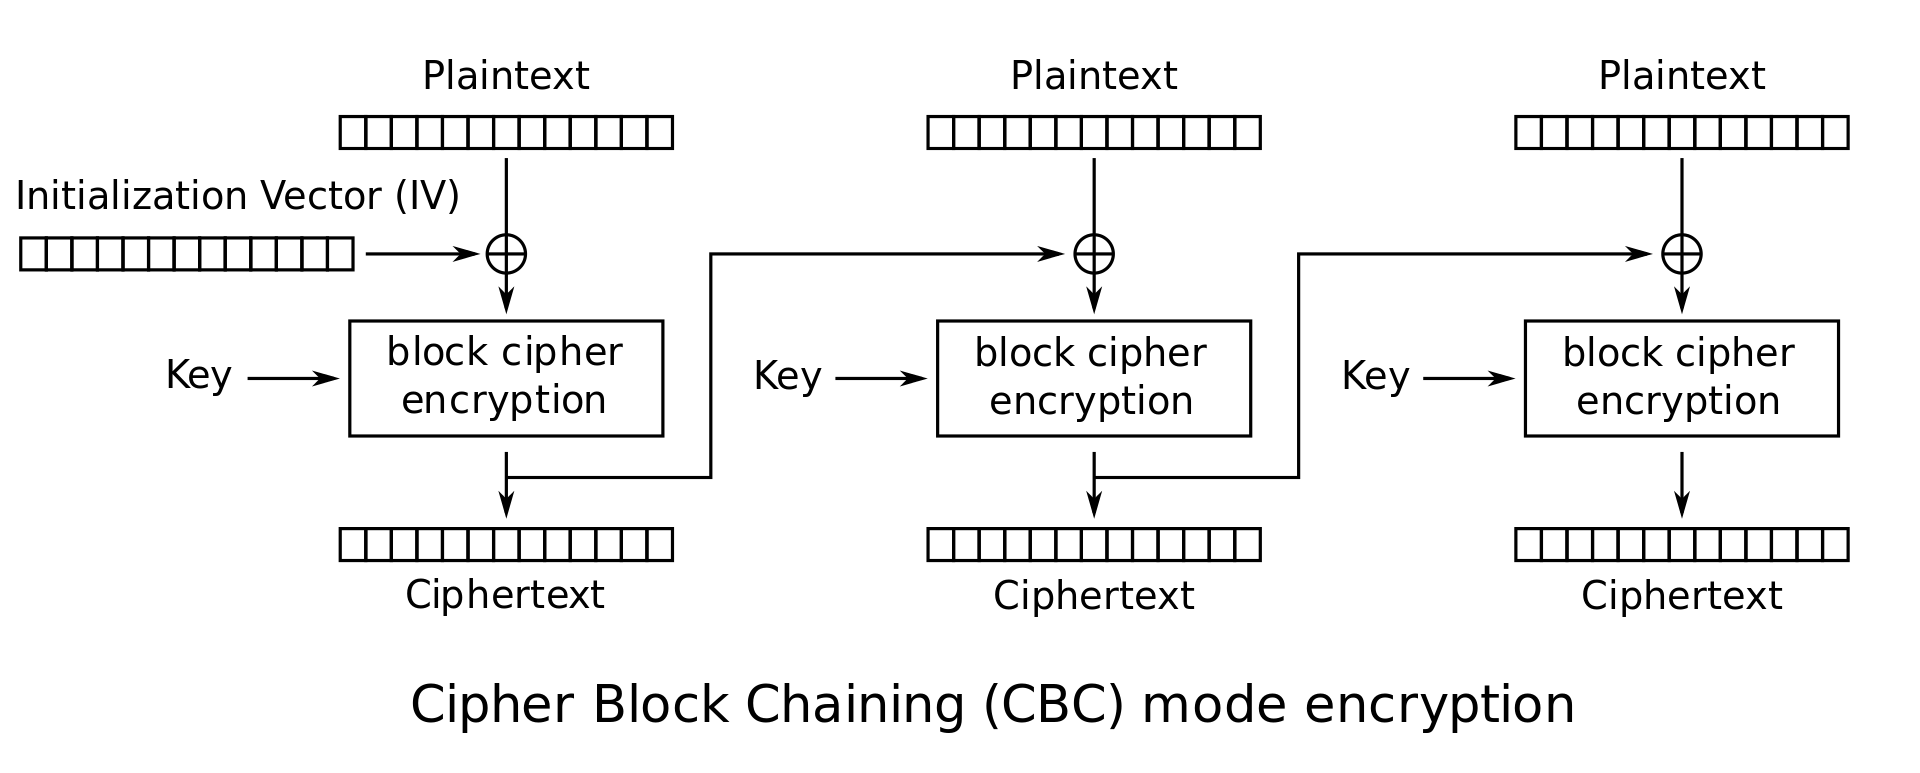
\includegraphics[width=1\linewidth]{rezim_cbc.png}
    \caption{Ukázka režimu CBC.}
\end{figure}

\subsection{Cipher Feedback (CFB)}

Režim CFB (\textit{šifrová zpětná vazba}) se liší oproti CBC v~prohození pořadí operací xor a šifrování -- nejprve se zašifruje předchozí šifrovaný blok (resp. inicializační vektor) a výsledek se xoruje s~otevřeným blokem. Toto prohození má významné implementační dopady: díky symetrii operace XOR vypadá dešifrovací funkce obdobně jako šifrovací. Šifruje pomaleji než CBC. Vstup není nutné zarovnávat. Plynou stejné nevýhody jako pro CBC.

\begin{equation}
\begin{aligned}
C_i &= E_K (C_{i-1}) \oplus P_i \\
P_i &= E_K (C_{i-1}) \oplus C_i \\
C_0 &= IV
\end{aligned}
\end{equation}

\begin{figure}[H]
    \centering
    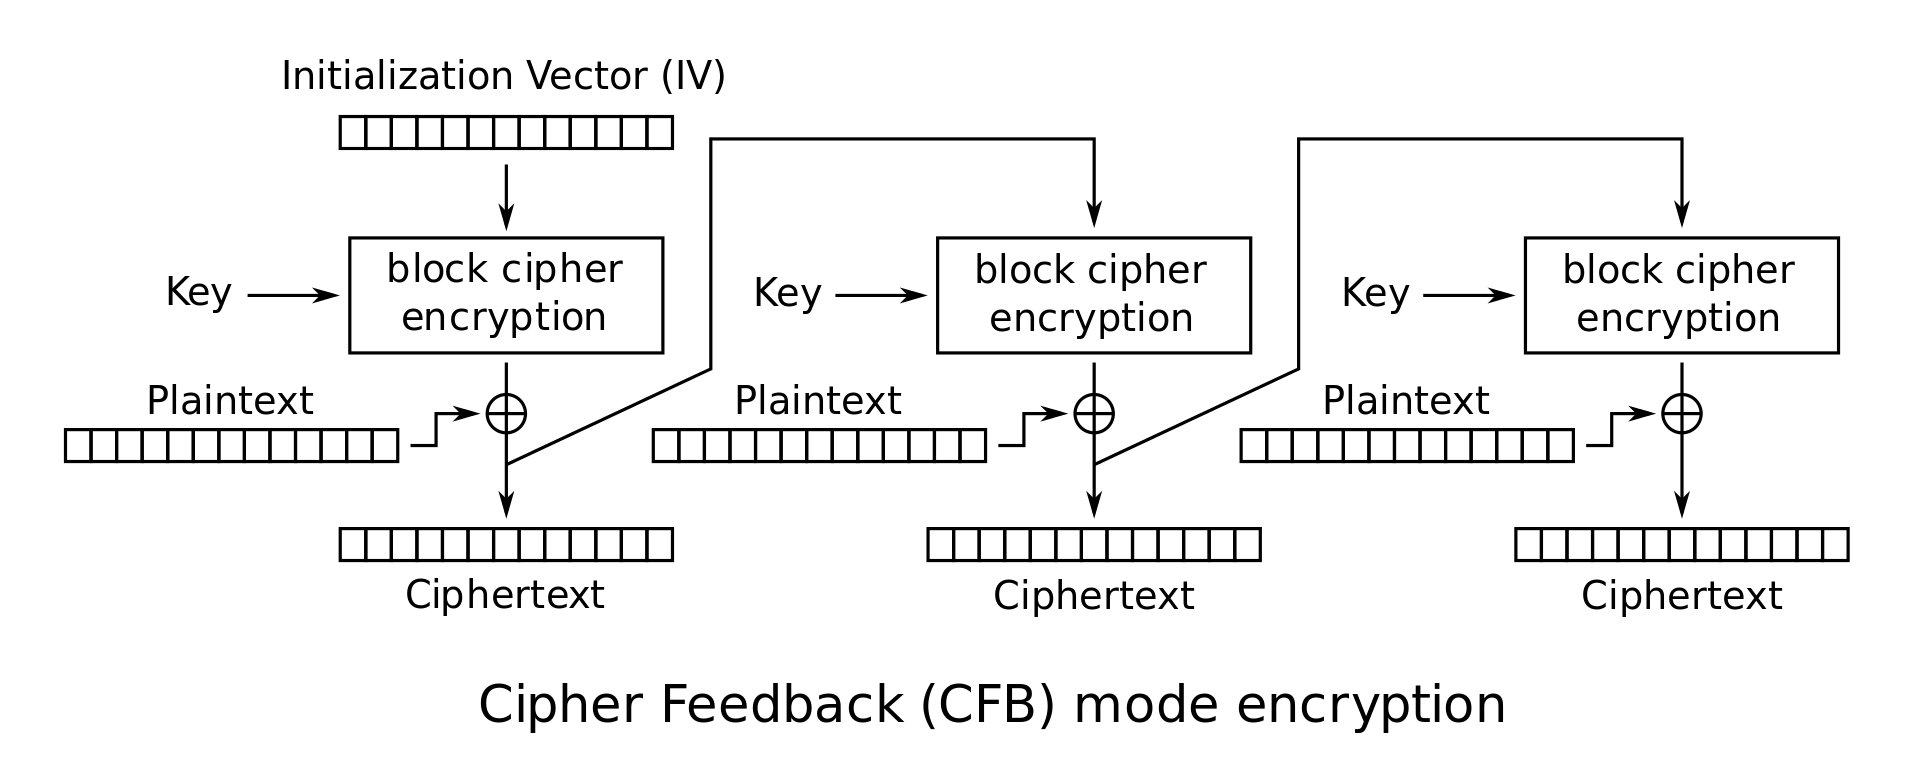
\includegraphics[width=1\linewidth]{rezim_cfb.png}
    \caption{Ukázka režimu CFB.}
\end{figure}

\subsection{Output Feedback (OFB)}

Režim OFB (\textit{výstupní zpětná vazba}) se liší od CFB pouze v~tom, kde bere zpětnou vazbu. Šifrování probíhá pouhým xorováním otevřeného bloku s~heslem, které je v~každém kroku zašifrováno použitou blokovou šifrou. První blok hesla je získán zašifrováním inicializačního vektoru. Režim převádí blokovou šifru na synchronní proudovou šifru.

\paragraph*{Slabina} Celý blok encryption je pouze generátor pseudonáhdon posloupnosti (je nezávislá na otevřeném nebo šifrovaném textu). To umožňuje Known Plaintext Attack. Z~toho plyne, že jedním klíčem není bezpečné šifrovat více než jednu zprávu.

\begin{equation}
\begin{aligned}
C_i &= E_K (C_{i-1}) \\
P_i &= P_i \oplus C_i \\
C_0 &= IV
\end{aligned}
\end{equation}

\begin{figure}[H]
    \centering
    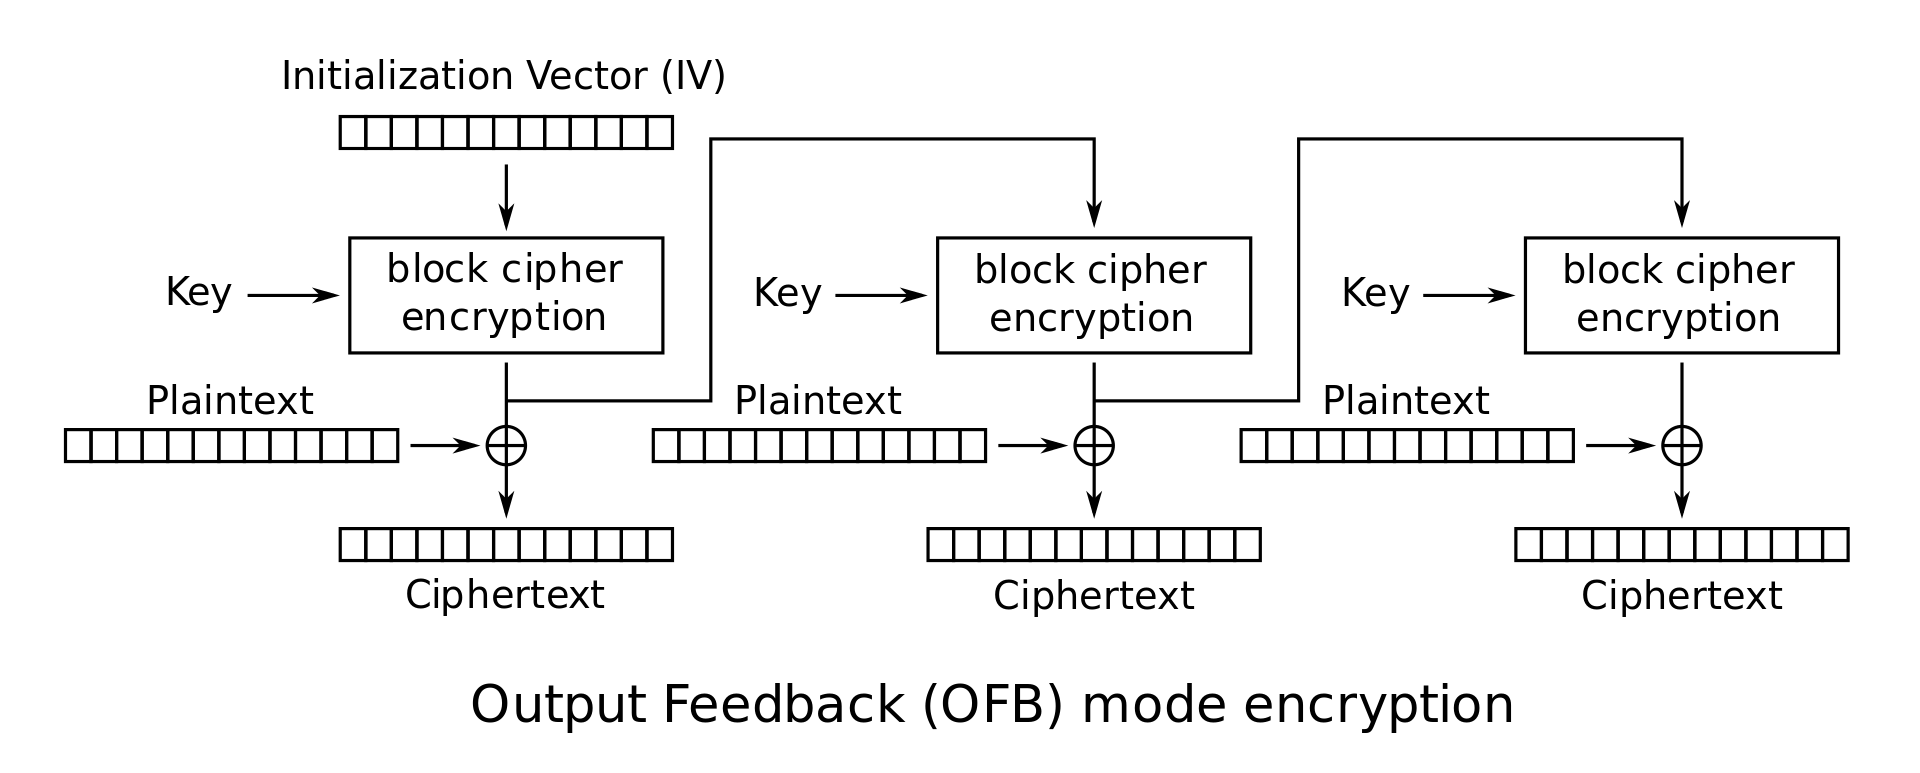
\includegraphics[width=1\linewidth]{rezim_ofb.png}
    \caption{Ukázka režimu OFB.}
\end{figure}

\subsection{Counter (CTR)}

Režim CTR (\uv{čítačový režim}) převádí stejně jako OFB blokovou šifru na synchronní proudovou. Heslo, se kterým se blok otevřeného textu xoruje, je však získáno zašifrováním čítače, který se každou iteraci zvětšuje o~pevně danou hodnotu, zpravidla o~1. Obsah čítače je opět před šifrováním nastaven inicializačním vektorem. Každý blok je šifrován nezávisle na ostatních, díky tomu je možné paralelizovat.

\begin{equation}
\begin{aligned}
CTR_i &= CTR_{i-1} + 1 \\
P_i &= P_i \oplus E_k(CTR_i) \\
CTR_0 &= IV
\end{aligned}
\end{equation}

\begin{figure}[H]
    \centering
    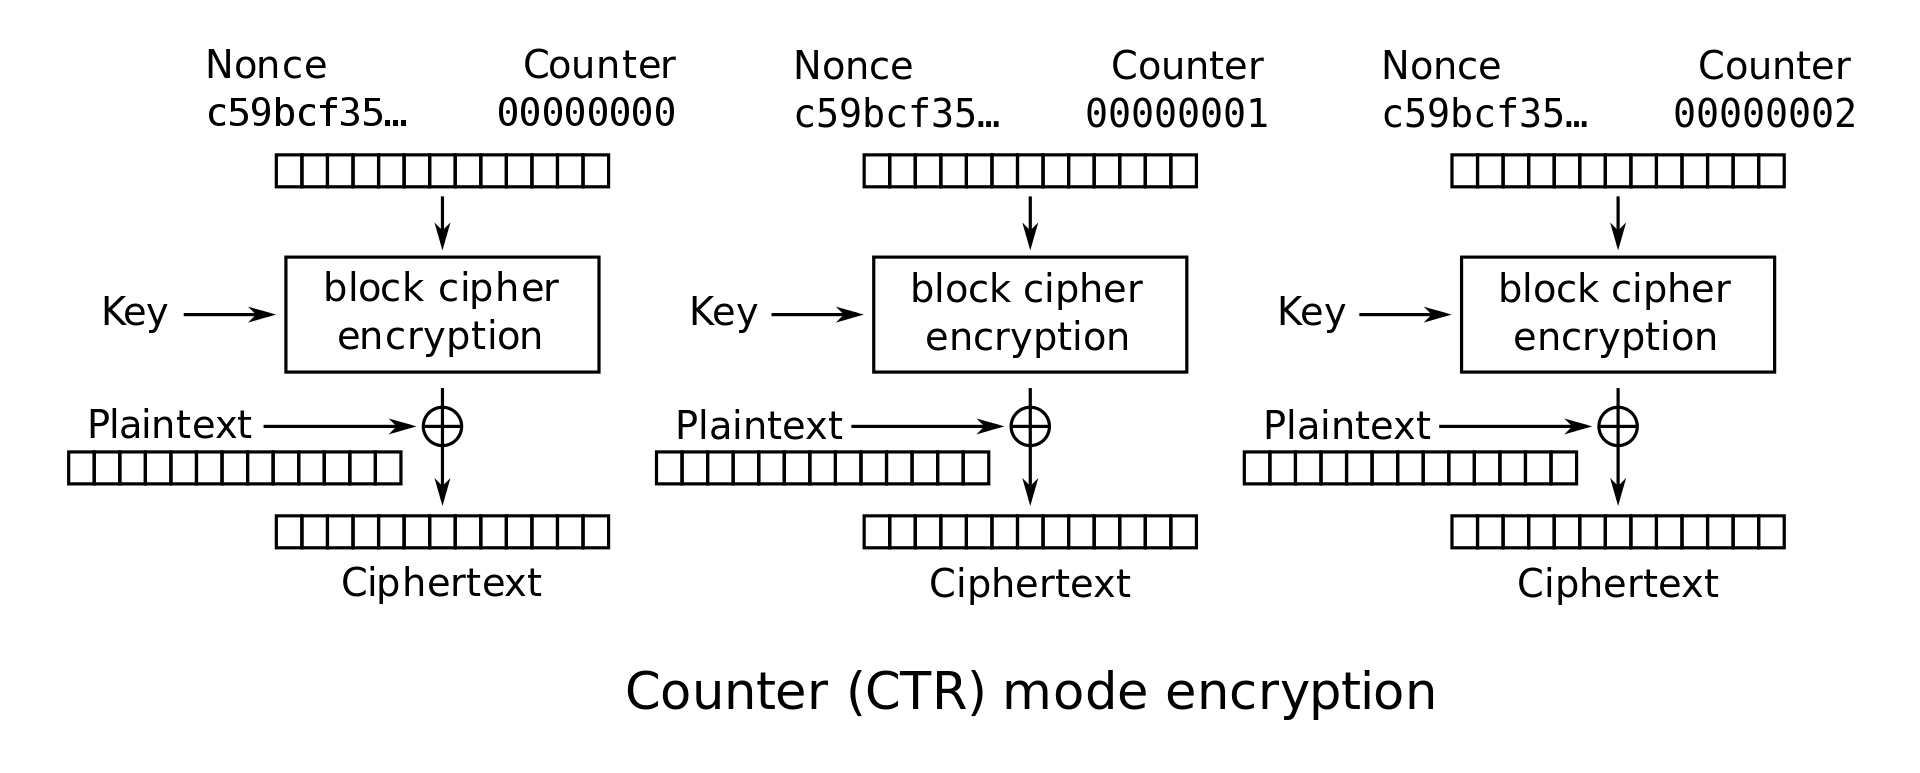
\includegraphics[width=1\linewidth]{rezim_ctr.png}
    \caption{Ukázka režimu CTR.}
\end{figure}

%%%%%%%%%%%%%%%%%%%%%%%%%%%%%%%%%%%%%%%%%%%%%%%%%%%%%%%%%%%%%%%%%%%%%%%%%%%%%%%%

\section{Proudové šifry}

Proudové šifry šifrují data jako \textit{proud} (stream), nejčastěji po jednotlivých bytech. Dešifrování vždy probíhá stejným způsobem. Proudové šifry jsou rychlejší než blokové šifry a pro implementaci potřebují jednodušší hardware.

\paragraph*{Problémy} \begin{compactitem}
    \item Nezajišťují samy o~sobě integritu.
    \item Na rozdíl od blokových šifer jsou náchylnější ke kryptoanalytickým útokům, pokud jsou nevhodně implementovány (počáteční stav nesmí být použit opakovaně)~--~\uv{problém s~inicializačním vektorem}.
\end{compactitem}

\begin{figure}[H]
    \centering
    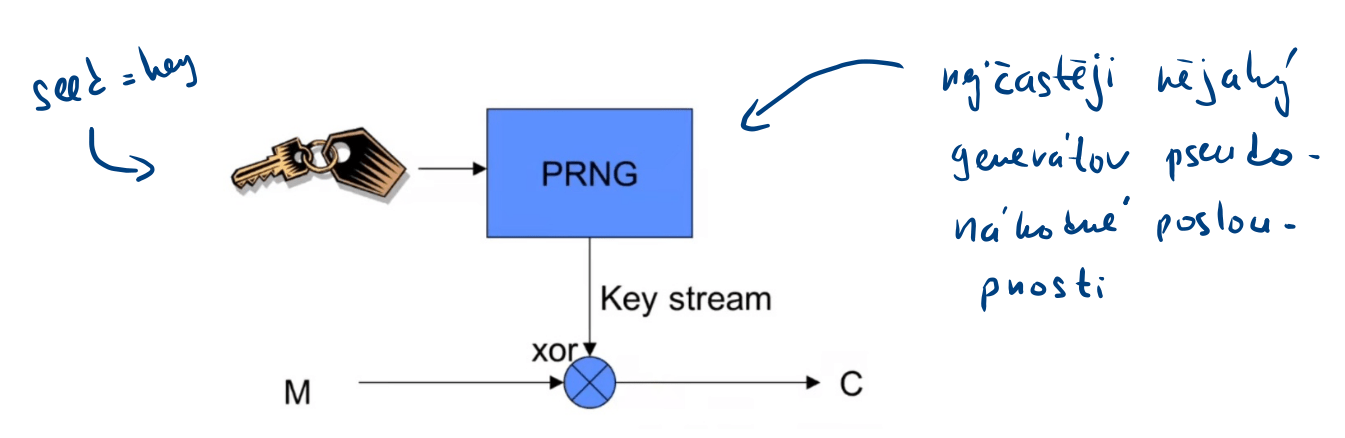
\includegraphics[width=1\linewidth]{proudove.png}
    \caption{Princip proudových šifer.}
\end{figure}

\subsection{Rozdělení proudových šifer}

\paragraph*{Synchronní proudové šifry} Proud pseudonáhodných čísel \textit{key stream} je generován nezávisle na vstupním textu nebo zašifrované zprávě. Poté dochází ke kombinaci vygenerovaných čísel se vstupujícím textem (k~zakódování) nebo se šifrovaným textem (k~dekódování). Nejběžnější formou kombinace keystreamu a vstupního textu je použití operace XOR. Např.: Vernamova šifra, DES v~režimu OFB. Pokud se průběhu dešifrování něco ztratí, je konec.

\begin{figure}[H]
    \centering
    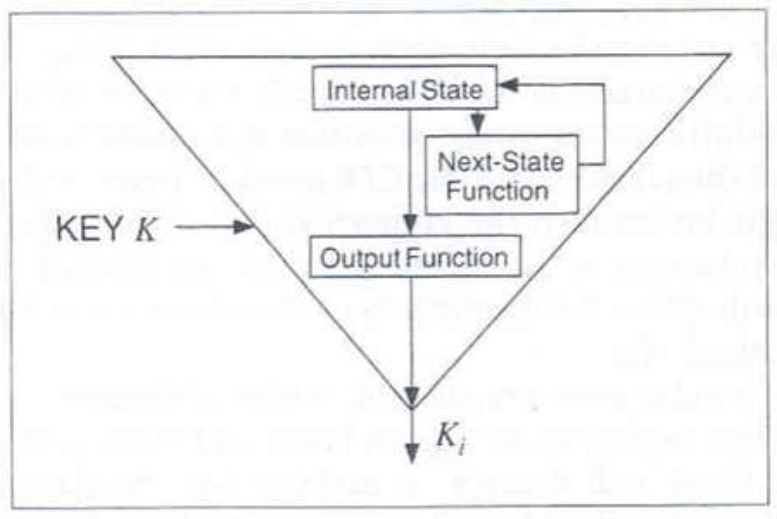
\includegraphics[width=0.5\linewidth]{proudova_synchronni.png}
    \caption{Princip synchronní proudové šifry.}
\end{figure}

\paragraph*{Samosynchronizující proudové šifry} Proud pseudonáhodných čísel \textit{key stream} závisí na pevném počtu předcházejících bytů šifrovaného (nebo otevřeného) textu. To znamená, že se šifra dokáže po chybě sama \textit{zotavit} (resynchronizovat)\footnote{Dnes se nesnážíme dešifrovat poškozená data, pokud nastane chyba v~přenosu, vyžádáme si data znovu.}. Např.: Vigenere Autokey, DES v~řežimu CFB.

\begin{figure}[H]
    \centering
    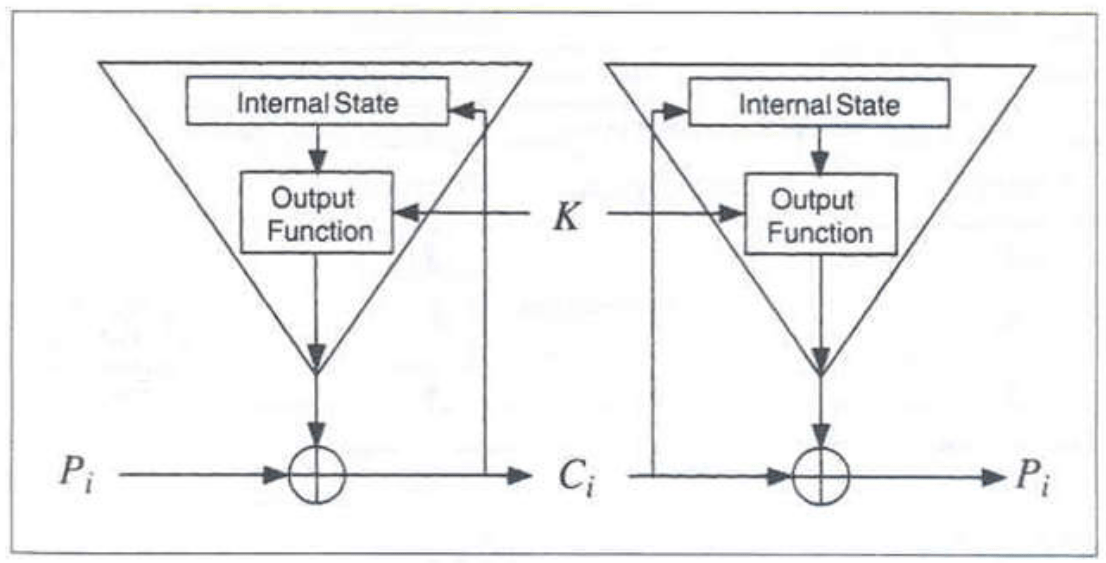
\includegraphics[width=0.75\linewidth]{proudova_samosynchronizujici.png}
    \caption{Princip samosynchronizující proudové šifry.}
\end{figure}

\subsection{Generátory PRNG}

Generátory PRNG (\textit{pseudo-random number generator}) generují pseudo-náhodnou pos\-loupnost (\textit{key stream}) z~malého klíče (\textit{seed}).

\paragraph*{Blokové šifry v~režimu OFB} Blokové šifry v~režimu OFB jsou pomalé.

\paragraph*{Linear Feedback Shift Registers (LSFR)} LFSR (posuvný registr s~lineární zpětnou vazbou) je posuvný registr, jehož výstup je lineárně závislý na jeho předchozích výstupech a stavu. Mějme \begin{compactitem}
    \item posuvný registr $R = (r_1, r_2, \dots, r_n)$,
    \item sekvenci zpětných vazeb $T = (t_1, t_2, \dots, t_n)$.
\end{compactitem}

\noindent Alternativně lze zapsat polynomem: $$
T(x) = x^n + x^{n-1} + \ldots + x + 1
$$

\begin{figure}[H]
    \centering
    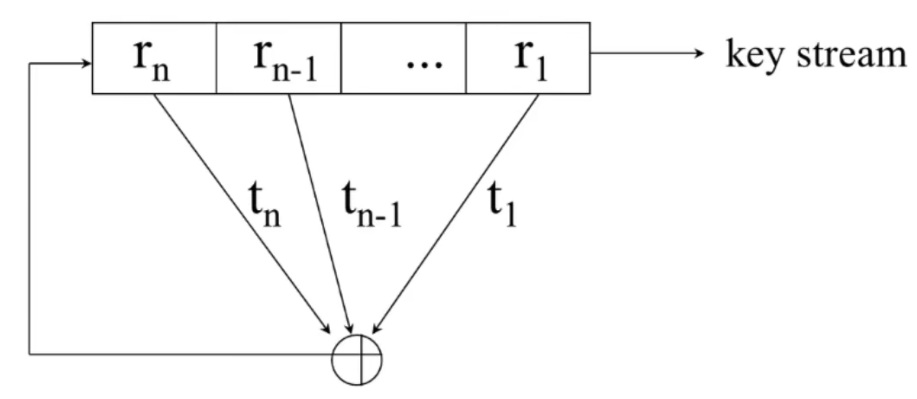
\includegraphics[width=0.6\linewidth]{lfsr.png}
    \caption{Příklad LFSR.}
\end{figure}

\paragraph*{Geffe generátor} Geffe generátor (kombinovaný generátor) je využití 2 a více LFSR propojených multiplexorem.

\begin{figure}[H]
    \centering
    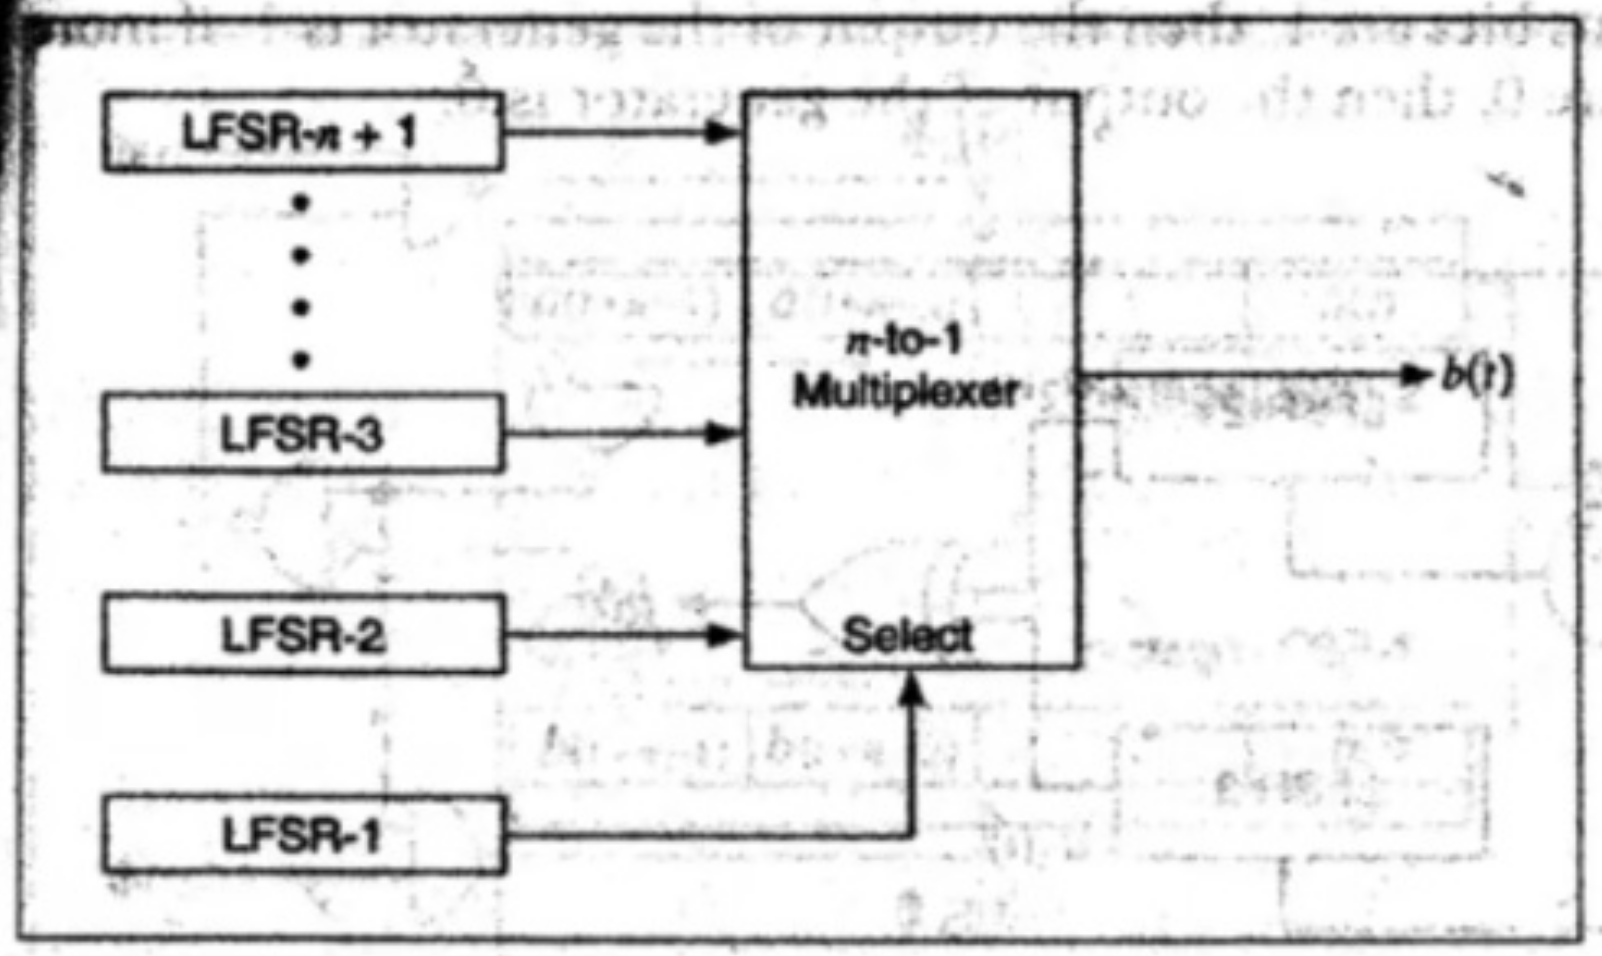
\includegraphics[width=0.75\linewidth]{geffe.png}
    \caption{Příklad Geffe generátoru.}
\end{figure}

\paragraph*{Stop and Go generátor} Stop and Go generátor je několik LSFR s~různým zdrojem hodin.

\begin{figure}[H]
    \centering
    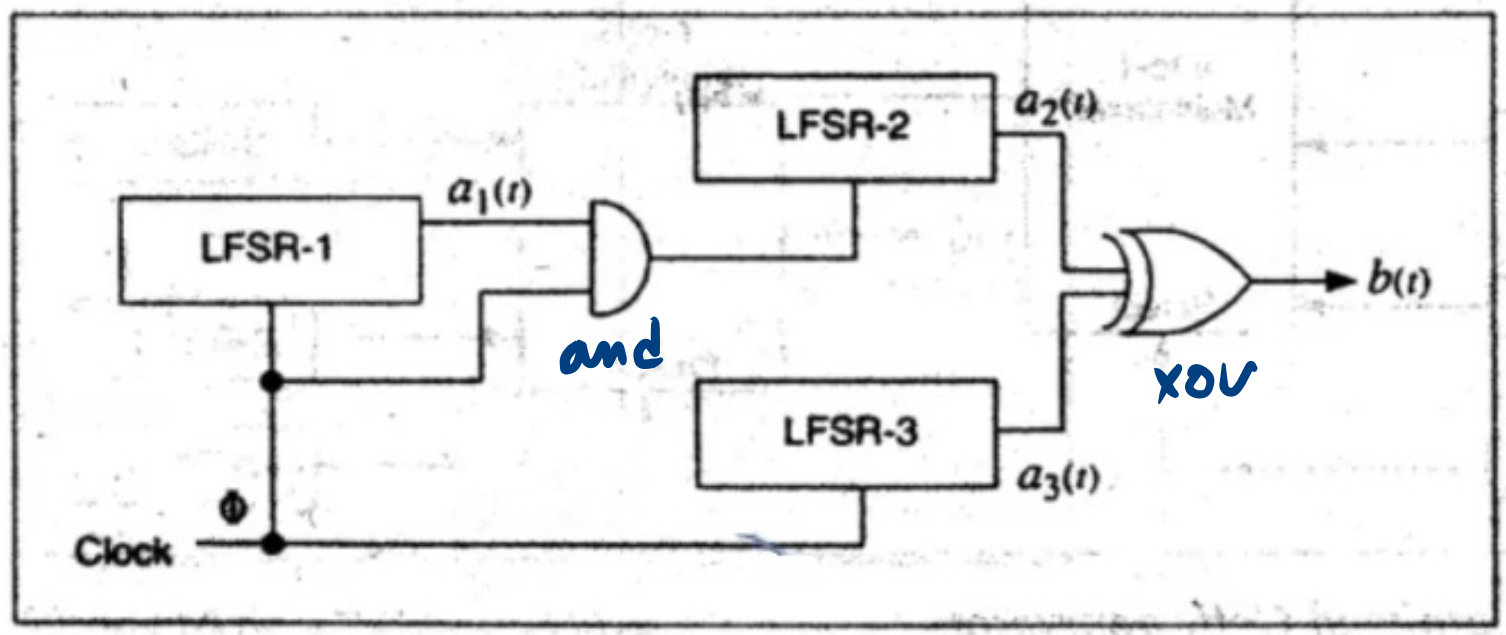
\includegraphics[width=0.8\linewidth]{stop_and_go.png}
    \caption{Příklad Stop and Go generátoru.}
\end{figure}
